% Options for packages loaded elsewhere
\PassOptionsToPackage{unicode}{hyperref}
\PassOptionsToPackage{hyphens}{url}
\PassOptionsToPackage{dvipsnames,svgnames,x11names}{xcolor}
%
\documentclass[
  letterpaper,
  DIV=11,
  numbers=noendperiod]{scrartcl}

\usepackage{amsmath,amssymb}
\usepackage{lmodern}
\usepackage{iftex}
\ifPDFTeX
  \usepackage[T1]{fontenc}
  \usepackage[utf8]{inputenc}
  \usepackage{textcomp} % provide euro and other symbols
\else % if luatex or xetex
  \usepackage{unicode-math}
  \defaultfontfeatures{Scale=MatchLowercase}
  \defaultfontfeatures[\rmfamily]{Ligatures=TeX,Scale=1}
\fi
% Use upquote if available, for straight quotes in verbatim environments
\IfFileExists{upquote.sty}{\usepackage{upquote}}{}
\IfFileExists{microtype.sty}{% use microtype if available
  \usepackage[]{microtype}
  \UseMicrotypeSet[protrusion]{basicmath} % disable protrusion for tt fonts
}{}
\makeatletter
\@ifundefined{KOMAClassName}{% if non-KOMA class
  \IfFileExists{parskip.sty}{%
    \usepackage{parskip}
  }{% else
    \setlength{\parindent}{0pt}
    \setlength{\parskip}{6pt plus 2pt minus 1pt}}
}{% if KOMA class
  \KOMAoptions{parskip=half}}
\makeatother
\usepackage{xcolor}
\setlength{\emergencystretch}{3em} % prevent overfull lines
\setcounter{secnumdepth}{-\maxdimen} % remove section numbering
% Make \paragraph and \subparagraph free-standing
\ifx\paragraph\undefined\else
  \let\oldparagraph\paragraph
  \renewcommand{\paragraph}[1]{\oldparagraph{#1}\mbox{}}
\fi
\ifx\subparagraph\undefined\else
  \let\oldsubparagraph\subparagraph
  \renewcommand{\subparagraph}[1]{\oldsubparagraph{#1}\mbox{}}
\fi

\usepackage{color}
\usepackage{fancyvrb}
\newcommand{\VerbBar}{|}
\newcommand{\VERB}{\Verb[commandchars=\\\{\}]}
\DefineVerbatimEnvironment{Highlighting}{Verbatim}{commandchars=\\\{\}}
% Add ',fontsize=\small' for more characters per line
\usepackage{framed}
\definecolor{shadecolor}{RGB}{241,243,245}
\newenvironment{Shaded}{\begin{snugshade}}{\end{snugshade}}
\newcommand{\AlertTok}[1]{\textcolor[rgb]{0.68,0.00,0.00}{#1}}
\newcommand{\AnnotationTok}[1]{\textcolor[rgb]{0.37,0.37,0.37}{#1}}
\newcommand{\AttributeTok}[1]{\textcolor[rgb]{0.40,0.45,0.13}{#1}}
\newcommand{\BaseNTok}[1]{\textcolor[rgb]{0.68,0.00,0.00}{#1}}
\newcommand{\BuiltInTok}[1]{\textcolor[rgb]{0.00,0.23,0.31}{#1}}
\newcommand{\CharTok}[1]{\textcolor[rgb]{0.13,0.47,0.30}{#1}}
\newcommand{\CommentTok}[1]{\textcolor[rgb]{0.37,0.37,0.37}{#1}}
\newcommand{\CommentVarTok}[1]{\textcolor[rgb]{0.37,0.37,0.37}{\textit{#1}}}
\newcommand{\ConstantTok}[1]{\textcolor[rgb]{0.56,0.35,0.01}{#1}}
\newcommand{\ControlFlowTok}[1]{\textcolor[rgb]{0.00,0.23,0.31}{#1}}
\newcommand{\DataTypeTok}[1]{\textcolor[rgb]{0.68,0.00,0.00}{#1}}
\newcommand{\DecValTok}[1]{\textcolor[rgb]{0.68,0.00,0.00}{#1}}
\newcommand{\DocumentationTok}[1]{\textcolor[rgb]{0.37,0.37,0.37}{\textit{#1}}}
\newcommand{\ErrorTok}[1]{\textcolor[rgb]{0.68,0.00,0.00}{#1}}
\newcommand{\ExtensionTok}[1]{\textcolor[rgb]{0.00,0.23,0.31}{#1}}
\newcommand{\FloatTok}[1]{\textcolor[rgb]{0.68,0.00,0.00}{#1}}
\newcommand{\FunctionTok}[1]{\textcolor[rgb]{0.28,0.35,0.67}{#1}}
\newcommand{\ImportTok}[1]{\textcolor[rgb]{0.00,0.46,0.62}{#1}}
\newcommand{\InformationTok}[1]{\textcolor[rgb]{0.37,0.37,0.37}{#1}}
\newcommand{\KeywordTok}[1]{\textcolor[rgb]{0.00,0.23,0.31}{#1}}
\newcommand{\NormalTok}[1]{\textcolor[rgb]{0.00,0.23,0.31}{#1}}
\newcommand{\OperatorTok}[1]{\textcolor[rgb]{0.37,0.37,0.37}{#1}}
\newcommand{\OtherTok}[1]{\textcolor[rgb]{0.00,0.23,0.31}{#1}}
\newcommand{\PreprocessorTok}[1]{\textcolor[rgb]{0.68,0.00,0.00}{#1}}
\newcommand{\RegionMarkerTok}[1]{\textcolor[rgb]{0.00,0.23,0.31}{#1}}
\newcommand{\SpecialCharTok}[1]{\textcolor[rgb]{0.37,0.37,0.37}{#1}}
\newcommand{\SpecialStringTok}[1]{\textcolor[rgb]{0.13,0.47,0.30}{#1}}
\newcommand{\StringTok}[1]{\textcolor[rgb]{0.13,0.47,0.30}{#1}}
\newcommand{\VariableTok}[1]{\textcolor[rgb]{0.07,0.07,0.07}{#1}}
\newcommand{\VerbatimStringTok}[1]{\textcolor[rgb]{0.13,0.47,0.30}{#1}}
\newcommand{\WarningTok}[1]{\textcolor[rgb]{0.37,0.37,0.37}{\textit{#1}}}

\providecommand{\tightlist}{%
  \setlength{\itemsep}{0pt}\setlength{\parskip}{0pt}}\usepackage{longtable,booktabs,array}
\usepackage{calc} % for calculating minipage widths
% Correct order of tables after \paragraph or \subparagraph
\usepackage{etoolbox}
\makeatletter
\patchcmd\longtable{\par}{\if@noskipsec\mbox{}\fi\par}{}{}
\makeatother
% Allow footnotes in longtable head/foot
\IfFileExists{footnotehyper.sty}{\usepackage{footnotehyper}}{\usepackage{footnote}}
\makesavenoteenv{longtable}
\usepackage{graphicx}
\makeatletter
\def\maxwidth{\ifdim\Gin@nat@width>\linewidth\linewidth\else\Gin@nat@width\fi}
\def\maxheight{\ifdim\Gin@nat@height>\textheight\textheight\else\Gin@nat@height\fi}
\makeatother
% Scale images if necessary, so that they will not overflow the page
% margins by default, and it is still possible to overwrite the defaults
% using explicit options in \includegraphics[width, height, ...]{}
\setkeys{Gin}{width=\maxwidth,height=\maxheight,keepaspectratio}
% Set default figure placement to htbp
\makeatletter
\def\fps@figure{htbp}
\makeatother

\usepackage{booktabs}
\usepackage{longtable}
\usepackage{array}
\usepackage{multirow}
\usepackage{wrapfig}
\usepackage{float}
\usepackage{colortbl}
\usepackage{pdflscape}
\usepackage{tabu}
\usepackage{threeparttable}
\usepackage{threeparttablex}
\usepackage[normalem]{ulem}
\usepackage{makecell}
\usepackage{xcolor}
\KOMAoption{captions}{tableheading}
\makeatletter
\makeatother
\makeatletter
\makeatother
\makeatletter
\@ifpackageloaded{caption}{}{\usepackage{caption}}
\AtBeginDocument{%
\ifdefined\contentsname
  \renewcommand*\contentsname{Table of contents}
\else
  \newcommand\contentsname{Table of contents}
\fi
\ifdefined\listfigurename
  \renewcommand*\listfigurename{List of Figures}
\else
  \newcommand\listfigurename{List of Figures}
\fi
\ifdefined\listtablename
  \renewcommand*\listtablename{List of Tables}
\else
  \newcommand\listtablename{List of Tables}
\fi
\ifdefined\figurename
  \renewcommand*\figurename{Figure}
\else
  \newcommand\figurename{Figure}
\fi
\ifdefined\tablename
  \renewcommand*\tablename{Table}
\else
  \newcommand\tablename{Table}
\fi
}
\@ifpackageloaded{float}{}{\usepackage{float}}
\floatstyle{ruled}
\@ifundefined{c@chapter}{\newfloat{codelisting}{h}{lop}}{\newfloat{codelisting}{h}{lop}[chapter]}
\floatname{codelisting}{Listing}
\newcommand*\listoflistings{\listof{codelisting}{List of Listings}}
\makeatother
\makeatletter
\@ifpackageloaded{caption}{}{\usepackage{caption}}
\@ifpackageloaded{subcaption}{}{\usepackage{subcaption}}
\makeatother
\makeatletter
\@ifpackageloaded{tcolorbox}{}{\usepackage[many]{tcolorbox}}
\makeatother
\makeatletter
\@ifundefined{shadecolor}{\definecolor{shadecolor}{rgb}{.97, .97, .97}}
\makeatother
\makeatletter
\makeatother
\ifLuaTeX
  \usepackage{selnolig}  % disable illegal ligatures
\fi
\IfFileExists{bookmark.sty}{\usepackage{bookmark}}{\usepackage{hyperref}}
\IfFileExists{xurl.sty}{\usepackage{xurl}}{} % add URL line breaks if available
\urlstyle{same} % disable monospaced font for URLs
\hypersetup{
  pdftitle={Exploratory N-Mixture/CMR - Pennsylvania},
  colorlinks=true,
  linkcolor={blue},
  filecolor={Maroon},
  citecolor={Blue},
  urlcolor={Blue},
  pdfcreator={LaTeX via pandoc}}

\title{Exploratory N-Mixture/CMR - Pennsylvania}
\author{}
\date{}

\begin{document}
\maketitle
\ifdefined\Shaded\renewenvironment{Shaded}{\begin{tcolorbox}[boxrule=0pt, breakable, borderline west={3pt}{0pt}{shadecolor}, sharp corners, enhanced, interior hidden, frame hidden]}{\end{tcolorbox}}\fi

\hypertarget{load-packages}{%
\subsection{Load Packages}\label{load-packages}}

\begin{Shaded}
\begin{Highlighting}[]
\ControlFlowTok{if}\NormalTok{ (}\SpecialCharTok{!}\FunctionTok{require}\NormalTok{(librarian))\{}
  \FunctionTok{install.packages}\NormalTok{(}\StringTok{"librarian"}\NormalTok{)}
  \FunctionTok{library}\NormalTok{(librarian)}
\NormalTok{\}}

\NormalTok{librarian}\SpecialCharTok{::}\FunctionTok{shelf}\NormalTok{(tidyverse, RPostgres, DBI, unmarked, here, lubridate, kableExtra)}
\end{Highlighting}
\end{Shaded}

\hypertarget{connect-to-survey_data-schema-in-ribbitr-database}{%
\subsection{\texorpdfstring{Connect to \texttt{survey\_data} schema in
\texttt{ribbitr}
database}{Connect to survey\_data schema in ribbitr database}}\label{connect-to-survey_data-schema-in-ribbitr-database}}

\begin{Shaded}
\begin{Highlighting}[]
\FunctionTok{tryCatch}\NormalTok{(\{}
\NormalTok{    drv }\OtherTok{\textless{}{-}} \FunctionTok{dbDriver}\NormalTok{(}\StringTok{"Postgres"}\NormalTok{)}
    \FunctionTok{print}\NormalTok{(}\StringTok{"Connecting to Database…"}\NormalTok{)}
\NormalTok{    connection }\OtherTok{\textless{}{-}} \FunctionTok{dbConnect}\NormalTok{(drv,}
                 \AttributeTok{dbname =} \FunctionTok{Sys.getenv}\NormalTok{(}\StringTok{"aws\_dbname"}\NormalTok{),}
                 \AttributeTok{host =} \FunctionTok{Sys.getenv}\NormalTok{(}\StringTok{"aws\_host"}\NormalTok{),}
                 \AttributeTok{port =} \FunctionTok{Sys.getenv}\NormalTok{(}\StringTok{"aws\_port"}\NormalTok{),}
                 \AttributeTok{user =} \FunctionTok{Sys.getenv}\NormalTok{(}\StringTok{"aws\_user"}\NormalTok{),}
                 \AttributeTok{password =} \FunctionTok{Sys.getenv}\NormalTok{(}\StringTok{"aws\_password"}\NormalTok{),}
                 \AttributeTok{timezone=}\ConstantTok{NULL}\NormalTok{)}
    \FunctionTok{print}\NormalTok{(}\StringTok{"Database Connected!"}\NormalTok{)}
\NormalTok{    \},}
    \AttributeTok{error=}\ControlFlowTok{function}\NormalTok{(cond) \{}
            \FunctionTok{print}\NormalTok{(}\StringTok{"Unable to connect to Database."}\NormalTok{)}
\NormalTok{    \})}

\CommentTok{\#search path}
\FunctionTok{dbExecute}\NormalTok{(connection, }\StringTok{"set search\_path to survey\_data"}\NormalTok{)}
\end{Highlighting}
\end{Shaded}

\hypertarget{query-2022-n-mix-penn-data}{%
\subsection{Query 2022 N-Mix Penn
data}\label{query-2022-n-mix-penn-data}}

\begin{Shaded}
\begin{Highlighting}[]
\CommentTok{\# Data}
\NormalTok{nmix\_q }\OtherTok{\textless{}{-}} \StringTok{"select r.region, s.site, v.date, v.survey\_time, s2.duration\_minutes, }
\StringTok{          c.species\_capture, c.capture\_type}
\StringTok{          from region r}
\StringTok{          join site s on r.region\_id = s.region\_id }
\StringTok{          full join visit v on s.site\_id = v.site\_id }
\StringTok{          join survey s2 on v.visit\_id = s2.visit\_id }
\StringTok{          join capture c on s2.survey\_id = c.survey\_id}
\StringTok{          where r.region = \textquotesingle{}pennsylvania\textquotesingle{}}
\StringTok{          and v.date \textgreater{} \textquotesingle{}2022{-}01{-}01\textquotesingle{};"}

\NormalTok{nmix\_raw\_data }\OtherTok{\textless{}{-}} \FunctionTok{dbGetQuery}\NormalTok{(connection, nmix\_q) }\SpecialCharTok{\%\textgreater{}\%} 
  \FunctionTok{select}\NormalTok{(}\SpecialCharTok{!}\FunctionTok{c}\NormalTok{(region, survey\_time, duration\_minutes)) }\SpecialCharTok{\%\textgreater{}\%} 
  \FunctionTok{arrange}\NormalTok{(date) }

\CommentTok{\#write\_csv(nmix\_raw\_data, here("data", "nmix\_raw\_data.csv"))}



\CommentTok{\# find all visits}
\NormalTok{visit\_nmix\_q }\OtherTok{\textless{}{-}} \StringTok{"select r.region, s.site, v.date, v.survey\_time}
\StringTok{                from region r}
\StringTok{                join site s on r.region\_id = s.region\_id }
\StringTok{                join visit v on s.site\_id = v.site\_id }
\StringTok{                where r.region = \textquotesingle{}pennsylvania\textquotesingle{}}
\StringTok{                and v.date \textgreater{} \textquotesingle{}2022{-}01{-}01\textquotesingle{};"}

\NormalTok{nmix\_raw\_visits }\OtherTok{\textless{}{-}}\FunctionTok{dbGetQuery}\NormalTok{(connection, visit\_nmix\_q) }\SpecialCharTok{\%\textgreater{}\%} 
  \FunctionTok{arrange}\NormalTok{(date) }\SpecialCharTok{\%\textgreater{}\%} 
  \FunctionTok{select}\NormalTok{(site, date)}


\CommentTok{\#write\_csv(nmix\_raw\_visits, here("data", "nmix\_raw\_visits.csv"))}
\end{Highlighting}
\end{Shaded}

\hypertarget{visualize-all-visits}{%
\subsection{Visualize all Visits}\label{visualize-all-visits}}

\begin{Shaded}
\begin{Highlighting}[]
\CommentTok{\#nmix\_raw\_visits \textless{}{-} read\_csv(here("data", "nmix\_raw\_visits.csv"))}
\CommentTok{\#nmix\_raw\_data \textless{}{-} read\_csv(here("data", "nmix\_raw\_data.csv"))}


\NormalTok{viz }\OtherTok{\textless{}{-}}\NormalTok{ nmix\_raw\_visits }\SpecialCharTok{\%\textgreater{}\%} 
  \FunctionTok{group\_by}\NormalTok{(site) }\SpecialCharTok{\%\textgreater{}\%} 
  \FunctionTok{summarise}\NormalTok{(}\AttributeTok{n =} \FunctionTok{n}\NormalTok{())}

\FunctionTok{ggplot}\NormalTok{(}\AttributeTok{data =}\NormalTok{ viz) }\SpecialCharTok{+}
  \FunctionTok{geom\_col}\NormalTok{(}\FunctionTok{aes}\NormalTok{(}\AttributeTok{x=}\NormalTok{site, }\AttributeTok{y =}\NormalTok{ n)) }\SpecialCharTok{+}
  \FunctionTok{ggtitle}\NormalTok{(}\StringTok{"Raw Visits"}\NormalTok{)}
\end{Highlighting}
\end{Shaded}

\begin{figure}[H]

{\centering 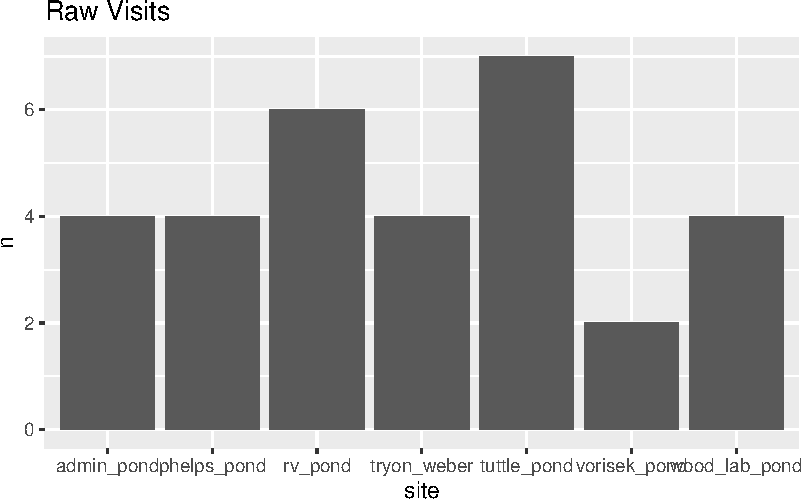
\includegraphics{cmr_penn_files/figure-pdf/unnamed-chunk-4-1.pdf}

}

\end{figure}

\newpage

\hypertarget{clean-up-species-list-with-counts}{%
\subsection{Clean up species list with
counts}\label{clean-up-species-list-with-counts}}

\hypertarget{filter-for-cmr-focal-species-and-summarize-species-counts.-then-populate-zeros-for-3-focal-species-into-the-data-set-for-visits-when-captures-did-not-occur.}{%
\paragraph{Filter for CMR focal species and summarize species counts.
Then populate zeros for 3 focal species into the data set for visits
when captures did not
occur.}\label{filter-for-cmr-focal-species-and-summarize-species-counts.-then-populate-zeros-for-3-focal-species-into-the-data-set-for-visits-when-captures-did-not-occur.}}

\begin{Shaded}
\begin{Highlighting}[]
\CommentTok{\# filter for CMR focal species and summarize counts}
\NormalTok{n\_mix\_mid\_clean\_up }\OtherTok{\textless{}{-}}\NormalTok{ nmix\_raw\_data }\SpecialCharTok{\%\textgreater{}\%} 
  \FunctionTok{filter}\NormalTok{(species\_capture }\SpecialCharTok{\%in\%} \FunctionTok{c}\NormalTok{(}\StringTok{"pseudacris\_crucifer"}\NormalTok{, }\StringTok{"rana\_catesbeiana"}\NormalTok{, }
                                \StringTok{"rana\_clamitans"}\NormalTok{)) }\SpecialCharTok{\%\textgreater{}\%} 
  \FunctionTok{mutate}\NormalTok{(}\AttributeTok{capture\_type =} \FunctionTok{if\_else}\NormalTok{(}\FunctionTok{is.na}\NormalTok{(capture\_type), }\StringTok{"new"}\NormalTok{, capture\_type)) }\SpecialCharTok{\%\textgreater{}\%} 
  \FunctionTok{group\_by}\NormalTok{(date, site, species\_capture) }\SpecialCharTok{\%\textgreater{}\%} 
  \FunctionTok{summarise}\NormalTok{(}\AttributeTok{n =} \FunctionTok{n}\NormalTok{()) }\SpecialCharTok{\%\textgreater{}\%} 
  \FunctionTok{ungroup}\NormalTok{() }

\CommentTok{\# populate zeros}
\NormalTok{nmix\_clean\_up }\OtherTok{\textless{}{-}}\NormalTok{ nmix\_raw\_visits }\SpecialCharTok{\%\textgreater{}\%} 
  \FunctionTok{left\_join}\NormalTok{(n\_mix\_mid\_clean\_up) }\SpecialCharTok{\%\textgreater{}\%}
  \FunctionTok{complete}\NormalTok{(}\FunctionTok{nesting}\NormalTok{(date, site), }
           \AttributeTok{species\_capture =} \FunctionTok{unique}\NormalTok{(n\_mix\_mid\_clean\_up}\SpecialCharTok{$}\NormalTok{species\_capture), }
           \AttributeTok{fill =} \FunctionTok{list}\NormalTok{(}\AttributeTok{n =} \DecValTok{0}\NormalTok{))}
\end{Highlighting}
\end{Shaded}

\begin{Shaded}
\begin{Highlighting}[]
\FunctionTok{kable}\NormalTok{(}\FunctionTok{head}\NormalTok{(nmix\_clean\_up, }\AttributeTok{n =} \DecValTok{15}\NormalTok{))}
\end{Highlighting}
\end{Shaded}

\begin{tabular}{l|l|l|r}
\hline
date & site & species\_capture & n\\
\hline
2022-05-04 & wood\_lab\_pond & pseudacris\_crucifer & 2\\
\hline
2022-05-04 & wood\_lab\_pond & rana\_catesbeiana & 2\\
\hline
2022-05-04 & wood\_lab\_pond & rana\_clamitans & 1\\
\hline
2022-05-05 & phelps\_pond & pseudacris\_crucifer & 4\\
\hline
2022-05-05 & phelps\_pond & rana\_catesbeiana & 4\\
\hline
2022-05-05 & phelps\_pond & rana\_clamitans & 7\\
\hline
2022-05-11 & admin\_pond & pseudacris\_crucifer & 4\\
\hline
2022-05-11 & admin\_pond & rana\_catesbeiana & 9\\
\hline
2022-05-11 & admin\_pond & rana\_clamitans & 5\\
\hline
2022-05-12 & rv\_pond & pseudacris\_crucifer & 16\\
\hline
2022-05-12 & rv\_pond & rana\_catesbeiana & 1\\
\hline
2022-05-12 & rv\_pond & rana\_clamitans & 0\\
\hline
2022-05-18 & admin\_pond & pseudacris\_crucifer & 2\\
\hline
2022-05-18 & admin\_pond & rana\_catesbeiana & 15\\
\hline
2022-05-18 & admin\_pond & rana\_clamitans & 3\\
\hline
\end{tabular}

\newpage

\hypertarget{rana_catesbeiana}{%
\subsection{rana\_catesbeiana}\label{rana_catesbeiana}}

\hypertarget{n-mixture-table-formatting}{%
\subsubsection{N-Mixture Table
formatting}\label{n-mixture-table-formatting}}

\hypertarget{filter-data-for-rana_catesbeiana-tally-the-numbner-of-visits-pivot-data-frame-into-correct-matrix-form-and-finally-populate-zeros-into-the-nas-if-sites-were-visited.}{%
\paragraph{\texorpdfstring{Filter data for \texttt{rana\_catesbeiana},
tally the numbner of visits, pivot data frame into correct matrix form,
and finally populate zeros into the NAs if sites were
visited.}{Filter data for rana\_catesbeiana, tally the numbner of visits, pivot data frame into correct matrix form, and finally populate zeros into the NAs if sites were visited.}}\label{filter-data-for-rana_catesbeiana-tally-the-numbner-of-visits-pivot-data-frame-into-correct-matrix-form-and-finally-populate-zeros-into-the-nas-if-sites-were-visited.}}

\begin{Shaded}
\begin{Highlighting}[]
\NormalTok{bull\_frog\_visits }\OtherTok{\textless{}{-}}\NormalTok{ nmix\_clean\_up }\SpecialCharTok{\%\textgreater{}\%} 
  \FunctionTok{select}\NormalTok{(site, date, species\_capture, n) }\SpecialCharTok{\%\textgreater{}\%} 
  \FunctionTok{filter}\NormalTok{(species\_capture }\SpecialCharTok{==} \StringTok{"rana\_catesbeiana"}\NormalTok{) }\SpecialCharTok{\%\textgreater{}\%} 
  \FunctionTok{select}\NormalTok{(}\SpecialCharTok{!}\NormalTok{species\_capture) }\SpecialCharTok{\%\textgreater{}\%} 
  \FunctionTok{group\_by}\NormalTok{(site) }\SpecialCharTok{\%\textgreater{}\%} 
  \FunctionTok{mutate}\NormalTok{(}\AttributeTok{n\_visit =} \FunctionTok{match}\NormalTok{(date, }\FunctionTok{unique}\NormalTok{(date)),}
         \AttributeTok{n\_visit =} \FunctionTok{paste0}\NormalTok{(}\StringTok{"visit\_"}\NormalTok{, n\_visit, }\AttributeTok{sep =} \StringTok{""}\NormalTok{)) }\SpecialCharTok{\%\textgreater{}\%} 
  \FunctionTok{select}\NormalTok{(}\SpecialCharTok{!}\NormalTok{date) }\SpecialCharTok{\%\textgreater{}\%} 
  \FunctionTok{ungroup}\NormalTok{() }\SpecialCharTok{\%\textgreater{}\%}
  \FunctionTok{pivot\_wider}\NormalTok{(}\AttributeTok{names\_from =} \FunctionTok{c}\NormalTok{(}\StringTok{"n\_visit"}\NormalTok{), }\AttributeTok{values\_from =} \FunctionTok{c}\NormalTok{(}\StringTok{"n"}\NormalTok{)) }\SpecialCharTok{\%\textgreater{}\%} 
  \FunctionTok{group\_by}\NormalTok{(site) }\SpecialCharTok{\%\textgreater{}\%} 
  \FunctionTok{mutate}\NormalTok{(}\FunctionTok{across}\NormalTok{(}\FunctionTok{contains}\NormalTok{(}\StringTok{"visit"}\NormalTok{), }
                \SpecialCharTok{\textasciitilde{}}\FunctionTok{ifelse}\NormalTok{(}\FunctionTok{is.na}\NormalTok{(.) }\SpecialCharTok{\&}
                          \SpecialCharTok{!}\FunctionTok{is.na}\NormalTok{(}\FunctionTok{lag}\NormalTok{(.)), }\DecValTok{0}\NormalTok{, .)))}



\FunctionTok{kable}\NormalTok{(bull\_frog\_visits)}
\end{Highlighting}
\end{Shaded}

\begin{tabular}{l|r|r|r|r|r|r|r}
\hline
site & visit\_1 & visit\_2 & visit\_3 & visit\_4 & visit\_5 & visit\_6 & visit\_7\\
\hline
wood\_lab\_pond & 2 & 4 & 3 & 0 & NA & NA & NA\\
\hline
phelps\_pond & 4 & 3 & 6 & 0 & NA & NA & NA\\
\hline
admin\_pond & 9 & 15 & 20 & 0 & NA & NA & NA\\
\hline
rv\_pond & 1 & 7 & 5 & 13 & 29 & 11 & NA\\
\hline
tuttle\_pond & 15 & 22 & 0 & 39 & 31 & 29 & 20\\
\hline
tryon\_weber & 0 & 0 & 0 & NA & NA & NA & NA\\
\hline
vorisek\_pond & 14 & 13 & NA & NA & NA & NA & NA\\
\hline
\end{tabular}

\hypertarget{static-n-mixture-models-no-covariates}{%
\subsubsection{static n-mixture models no
covariates}\label{static-n-mixture-models-no-covariates}}

\begin{Shaded}
\begin{Highlighting}[]
\NormalTok{bull\_frog\_unmarked\_nmixture }\OtherTok{\textless{}{-}}\NormalTok{ bull\_frog\_visits }\SpecialCharTok{\%\textgreater{}\%} 
  \FunctionTok{ungroup}\NormalTok{() }\SpecialCharTok{\%\textgreater{}\%} 
  \FunctionTok{select}\NormalTok{(}\SpecialCharTok{!}\NormalTok{site)}


\NormalTok{umf }\OtherTok{\textless{}{-}} \FunctionTok{unmarkedFramePCount}\NormalTok{(}\AttributeTok{y =}\NormalTok{ bull\_frog\_unmarked\_nmixture)}

\FunctionTok{summary}\NormalTok{(umf)}
\end{Highlighting}
\end{Shaded}

\begin{verbatim}
unmarkedFrame Object

7 sites
Maximum number of observations per site: 7 
Mean number of observations per site: 4.29 
Sites with at least one detection: 6 

Tabulation of y observations:
   0    1    2    3    4    5    6    7    9   11   13   14   15   20   22   29 
   7    1    1    2    2    1    1    1    1    1    2    1    2    2    1    2 
  31   39 <NA> 
   1    1   19 
\end{verbatim}

\begin{Shaded}
\begin{Highlighting}[]
\NormalTok{fm1 }\OtherTok{\textless{}{-}} \FunctionTok{pcount}\NormalTok{( }\SpecialCharTok{\textasciitilde{}} \DecValTok{1} \SpecialCharTok{\textasciitilde{}} \DecValTok{1}\NormalTok{, }
               \AttributeTok{data =}\NormalTok{ umf, }
               \AttributeTok{engine =} \StringTok{"R"}\NormalTok{)}
\end{Highlighting}
\end{Shaded}

\begin{verbatim}
Warning in pcount(~1 ~ 1, data = umf, engine = "R"): K was not specified and was
set to 139.
\end{verbatim}

\begin{Shaded}
\begin{Highlighting}[]
\FunctionTok{summary}\NormalTok{(fm1)}
\end{Highlighting}
\end{Shaded}

\begin{verbatim}

Call:
pcount(formula = ~1 ~ 1, data = umf, engine = "R")

Abundance (log-scale):
 Estimate    SE    z  P(>|z|)
     3.71 0.196 18.9 6.13e-80

Detection (logit-scale):
 Estimate    SE     z  P(>|z|)
     -1.2 0.236 -5.06 4.14e-07

AIC: 401.9176 
Number of sites: 7
optim convergence code: 0
optim iterations: 24 
Bootstrap iterations: 0 
\end{verbatim}

\begin{Shaded}
\begin{Highlighting}[]
\FunctionTok{backTransform}\NormalTok{(fm1, }\StringTok{"state"}\NormalTok{)}
\end{Highlighting}
\end{Shaded}

\begin{verbatim}
Backtransformed linear combination(s) of Abundance estimate(s)

 Estimate   SE LinComb (Intercept)
     40.7 7.97    3.71           1

Transformation: exp 
\end{verbatim}

\begin{Shaded}
\begin{Highlighting}[]
\FunctionTok{backTransform}\NormalTok{(fm1, }\StringTok{"det"}\NormalTok{)}
\end{Highlighting}
\end{Shaded}

\begin{verbatim}
Backtransformed linear combination(s) of Detection estimate(s)

 Estimate     SE LinComb (Intercept)
    0.232 0.0421    -1.2           1

Transformation: logistic 
\end{verbatim}

\hypertarget{assuming-the-sites-and-enviro-variables-are-exactly-the-same-we-can-say-there-is-40.7--7.9-frogs-at-each-site-with-23-chance-of-detecting-each-individual.}{%
\paragraph{Assuming the sites and enviro variables are exactly the same
we can say there is 40.7 +-7.9 frogs at each site with 23 \% chance of
detecting each
individual.}\label{assuming-the-sites-and-enviro-variables-are-exactly-the-same-we-can-say-there-is-40.7--7.9-frogs-at-each-site-with-23-chance-of-detecting-each-individual.}}

\newpage

\(~\)

\hypertarget{pseudacris_crucifer}{%
\subsection{pseudacris\_crucifer}\label{pseudacris_crucifer}}

\hypertarget{n-mixture-table-formatting-1}{%
\subsubsection{N-Mixture Table
formatting}\label{n-mixture-table-formatting-1}}

\hypertarget{filter-data-for-pseudacris_crucifer-tally-the-numbner-of-visits-pivot-data-frame-into-correct-matrix-form-and-finally-populate-zeros-into-the-nas-if-sites-were-visited.}{%
\paragraph{\texorpdfstring{Filter data for
\texttt{pseudacris\_crucifer}, tally the numbner of visits, pivot data
frame into correct matrix form, and finally populate zeros into the NAs
if sites were
visited.}{Filter data for pseudacris\_crucifer, tally the numbner of visits, pivot data frame into correct matrix form, and finally populate zeros into the NAs if sites were visited.}}\label{filter-data-for-pseudacris_crucifer-tally-the-numbner-of-visits-pivot-data-frame-into-correct-matrix-form-and-finally-populate-zeros-into-the-nas-if-sites-were-visited.}}

\begin{Shaded}
\begin{Highlighting}[]
\NormalTok{peep\_frog\_visits }\OtherTok{\textless{}{-}}\NormalTok{ nmix\_clean\_up }\SpecialCharTok{\%\textgreater{}\%} 
  \FunctionTok{select}\NormalTok{(site, date, species\_capture, n) }\SpecialCharTok{\%\textgreater{}\%} 
  \FunctionTok{filter}\NormalTok{(species\_capture }\SpecialCharTok{==} \StringTok{"pseudacris\_crucifer"}\NormalTok{) }\SpecialCharTok{\%\textgreater{}\%} 
  \FunctionTok{select}\NormalTok{(}\SpecialCharTok{!}\NormalTok{species\_capture) }\SpecialCharTok{\%\textgreater{}\%} 
  \FunctionTok{group\_by}\NormalTok{(site) }\SpecialCharTok{\%\textgreater{}\%} 
  \FunctionTok{mutate}\NormalTok{(}\AttributeTok{n\_visit =} \FunctionTok{match}\NormalTok{(date, }\FunctionTok{unique}\NormalTok{(date)),}
         \AttributeTok{n\_visit =} \FunctionTok{paste0}\NormalTok{(}\StringTok{"visit\_"}\NormalTok{, n\_visit, }\AttributeTok{sep =} \StringTok{""}\NormalTok{)) }\SpecialCharTok{\%\textgreater{}\%} 
  \FunctionTok{select}\NormalTok{(}\SpecialCharTok{!}\NormalTok{date) }\SpecialCharTok{\%\textgreater{}\%} 
  \FunctionTok{ungroup}\NormalTok{() }\SpecialCharTok{\%\textgreater{}\%}
  \FunctionTok{pivot\_wider}\NormalTok{(}\AttributeTok{names\_from =} \FunctionTok{c}\NormalTok{(}\StringTok{"n\_visit"}\NormalTok{), }\AttributeTok{values\_from =} \FunctionTok{c}\NormalTok{(}\StringTok{"n"}\NormalTok{))}\SpecialCharTok{\%\textgreater{}\%} 
  \FunctionTok{group\_by}\NormalTok{(site) }\SpecialCharTok{\%\textgreater{}\%} 
  \FunctionTok{mutate}\NormalTok{(}\FunctionTok{across}\NormalTok{(}\FunctionTok{contains}\NormalTok{(}\StringTok{"visit"}\NormalTok{), }
                \SpecialCharTok{\textasciitilde{}}\FunctionTok{ifelse}\NormalTok{(}\FunctionTok{is.na}\NormalTok{(.) }\SpecialCharTok{\&}
                          \SpecialCharTok{!}\FunctionTok{is.na}\NormalTok{(}\FunctionTok{lag}\NormalTok{(.)), }\DecValTok{0}\NormalTok{, .)))}


\FunctionTok{kable}\NormalTok{(peep\_frog\_visits)}
\end{Highlighting}
\end{Shaded}

\begin{tabular}{l|r|r|r|r|r|r|r}
\hline
site & visit\_1 & visit\_2 & visit\_3 & visit\_4 & visit\_5 & visit\_6 & visit\_7\\
\hline
wood\_lab\_pond & 2 & 0 & 0 & 0 & NA & NA & NA\\
\hline
phelps\_pond & 4 & 0 & 0 & 0 & NA & NA & NA\\
\hline
admin\_pond & 4 & 2 & 3 & 1 & NA & NA & NA\\
\hline
rv\_pond & 16 & 0 & 0 & 0 & 0 & 0 & NA\\
\hline
tuttle\_pond & 0 & 0 & 0 & 0 & 0 & 0 & 0\\
\hline
tryon\_weber & 0 & 0 & 0 & NA & NA & NA & NA\\
\hline
vorisek\_pond & 0 & 0 & NA & NA & NA & NA & NA\\
\hline
\end{tabular}

\hypertarget{static-n-mixture-model-no-covariates}{%
\subsubsection{static n-mixture model no
covariates}\label{static-n-mixture-model-no-covariates}}

\begin{Shaded}
\begin{Highlighting}[]
\NormalTok{peep\_unmarked\_nmixture }\OtherTok{\textless{}{-}}\NormalTok{ peep\_frog\_visits }\SpecialCharTok{\%\textgreater{}\%} 
  \FunctionTok{ungroup}\NormalTok{() }\SpecialCharTok{\%\textgreater{}\%} 
  \CommentTok{\#filter(capture\_type == "new") \%\textgreater{}\% }
  \FunctionTok{select}\NormalTok{(}\SpecialCharTok{!}\FunctionTok{c}\NormalTok{(site)) }


\NormalTok{umf }\OtherTok{\textless{}{-}} \FunctionTok{unmarkedFramePCount}\NormalTok{(}\AttributeTok{y =}\NormalTok{ peep\_unmarked\_nmixture)}

\FunctionTok{summary}\NormalTok{(umf)}
\end{Highlighting}
\end{Shaded}

\begin{verbatim}
unmarkedFrame Object

7 sites
Maximum number of observations per site: 7 
Mean number of observations per site: 4.29 
Sites with at least one detection: 4 

Tabulation of y observations:
   0    1    2    3    4   16 <NA> 
  23    1    2    1    2    1   19 
\end{verbatim}

\begin{Shaded}
\begin{Highlighting}[]
\NormalTok{fm1 }\OtherTok{\textless{}{-}} \FunctionTok{pcount}\NormalTok{(}\SpecialCharTok{\textasciitilde{}}\DecValTok{1} \SpecialCharTok{\textasciitilde{}}\DecValTok{1}\NormalTok{, }\AttributeTok{data =}\NormalTok{ umf)}
\end{Highlighting}
\end{Shaded}

\begin{verbatim}
Warning in pcount(~1 ~ 1, data = umf): K was not specified and was set to 116.
\end{verbatim}

\begin{Shaded}
\begin{Highlighting}[]
\FunctionTok{backTransform}\NormalTok{(fm1, }\StringTok{"state"}\NormalTok{) }
\end{Highlighting}
\end{Shaded}

\begin{verbatim}
Backtransformed linear combination(s) of Abundance estimate(s)

 Estimate   SE LinComb (Intercept)
     85.8 24.4    4.45           1

Transformation: exp 
\end{verbatim}

\begin{Shaded}
\begin{Highlighting}[]
\FunctionTok{backTransform}\NormalTok{(fm1, }\StringTok{"det"}\NormalTok{)}
\end{Highlighting}
\end{Shaded}

\begin{verbatim}
Backtransformed linear combination(s) of Detection estimate(s)

 Estimate      SE LinComb (Intercept)
   0.0124 0.00411   -4.38           1

Transformation: logistic 
\end{verbatim}

\hypertarget{assuming-the-sites-and-enviro-variables-are-exactly-the-same-we-can-estimate-there-is-85.7--24.4-frogs-at-each-site-with-a-1.2-chance-of-detecting-each-individual.}{%
\paragraph{Assuming the sites and enviro variables are exactly the same
we can estimate there is 85.7 +-24.4 frogs at each site with a 1.2\%
chance of detecting each
individual.}\label{assuming-the-sites-and-enviro-variables-are-exactly-the-same-we-can-estimate-there-is-85.7--24.4-frogs-at-each-site-with-a-1.2-chance-of-detecting-each-individual.}}

\newpage

\hypertarget{rana_clamitans}{%
\subsection{rana\_clamitans}\label{rana_clamitans}}

\hypertarget{n-mixture-table-formatting-2}{%
\subsubsection{N-Mixture Table
Formatting}\label{n-mixture-table-formatting-2}}

\hypertarget{filter-data-for-rana_clamitans-tally-the-numbner-of-visits-pivot-data-frame-into-correct-matrix-form-and-finally-populate-zeros-into-the-nas-if-sites-were-visited.}{%
\paragraph{\texorpdfstring{Filter data for \texttt{rana\_clamitans},
tally the numbner of visits, pivot data frame into correct matrix form,
and finally populate zeros into the NAs if sites were
visited.}{Filter data for rana\_clamitans, tally the numbner of visits, pivot data frame into correct matrix form, and finally populate zeros into the NAs if sites were visited.}}\label{filter-data-for-rana_clamitans-tally-the-numbner-of-visits-pivot-data-frame-into-correct-matrix-form-and-finally-populate-zeros-into-the-nas-if-sites-were-visited.}}

\begin{Shaded}
\begin{Highlighting}[]
\NormalTok{green\_frog\_visits }\OtherTok{\textless{}{-}}\NormalTok{ nmix\_clean\_up }\SpecialCharTok{\%\textgreater{}\%} 
  \FunctionTok{select}\NormalTok{(site, date, species\_capture, n) }\SpecialCharTok{\%\textgreater{}\%} 
  \FunctionTok{filter}\NormalTok{(species\_capture }\SpecialCharTok{==} \StringTok{"rana\_clamitans"}\NormalTok{) }\SpecialCharTok{\%\textgreater{}\%} 
  \CommentTok{\#select(!species\_capture) \%\textgreater{}\% }
  \FunctionTok{group\_by}\NormalTok{(site) }\SpecialCharTok{\%\textgreater{}\%} 
  \FunctionTok{mutate}\NormalTok{(}\AttributeTok{n\_visit =} \FunctionTok{match}\NormalTok{(date, }\FunctionTok{unique}\NormalTok{(date)),}
         \AttributeTok{n\_visit =} \FunctionTok{paste0}\NormalTok{(}\StringTok{"visit\_"}\NormalTok{, n\_visit, }\AttributeTok{sep =} \StringTok{""}\NormalTok{)) }\SpecialCharTok{\%\textgreater{}\%} 
  \FunctionTok{select}\NormalTok{(}\SpecialCharTok{!}\NormalTok{date) }\SpecialCharTok{\%\textgreater{}\%} 
  \FunctionTok{ungroup}\NormalTok{() }\SpecialCharTok{\%\textgreater{}\%}
  \FunctionTok{group\_by}\NormalTok{(site, n\_visit, ) }\SpecialCharTok{\%\textgreater{}\%} 
  \FunctionTok{summarise}\NormalTok{(}\AttributeTok{n =} \FunctionTok{sum}\NormalTok{(n)) }\SpecialCharTok{\%\textgreater{}\%} 
  \FunctionTok{ungroup}\NormalTok{() }\SpecialCharTok{\%\textgreater{}\%} 
  \FunctionTok{pivot\_wider}\NormalTok{(}\AttributeTok{names\_from =} \FunctionTok{c}\NormalTok{(}\StringTok{"n\_visit"}\NormalTok{), }\AttributeTok{values\_from =} \FunctionTok{c}\NormalTok{(}\StringTok{"n"}\NormalTok{)) }\SpecialCharTok{\%\textgreater{}\%} 
  \CommentTok{\#add\_row(site = "phelps\_pond", capture\_type = "recapture") \%\textgreater{}\% }
  \FunctionTok{group\_by}\NormalTok{(site) }\SpecialCharTok{\%\textgreater{}\%} 
  \FunctionTok{mutate}\NormalTok{(}\FunctionTok{across}\NormalTok{(}\FunctionTok{contains}\NormalTok{(}\StringTok{"visit"}\NormalTok{), }
                \SpecialCharTok{\textasciitilde{}}\FunctionTok{ifelse}\NormalTok{(}\FunctionTok{is.na}\NormalTok{(.) }\SpecialCharTok{\&}
                          \SpecialCharTok{!}\FunctionTok{is.na}\NormalTok{(}\FunctionTok{lag}\NormalTok{(.)), }\DecValTok{0}\NormalTok{, .))) }
\end{Highlighting}
\end{Shaded}

\begin{verbatim}
`summarise()` has grouped output by 'site'. You can override using the
`.groups` argument.
\end{verbatim}

\hypertarget{static-n-mixture-with-no-co-variates}{%
\subsubsection{static n-mixture with no
co-variates}\label{static-n-mixture-with-no-co-variates}}

\begin{Shaded}
\begin{Highlighting}[]
\NormalTok{green\_frog\_unmarked\_nmixture }\OtherTok{\textless{}{-}}\NormalTok{ green\_frog\_visits }\SpecialCharTok{\%\textgreater{}\%} 
  \FunctionTok{ungroup}\NormalTok{() }\SpecialCharTok{\%\textgreater{}\%} 
  \FunctionTok{select}\NormalTok{(}\SpecialCharTok{!}\FunctionTok{c}\NormalTok{(site)) }


\NormalTok{umf }\OtherTok{\textless{}{-}} \FunctionTok{unmarkedFramePCount}\NormalTok{(}\AttributeTok{y =}\NormalTok{ green\_frog\_unmarked\_nmixture)}

\FunctionTok{summary}\NormalTok{(umf)}
\end{Highlighting}
\end{Shaded}

\begin{verbatim}
unmarkedFrame Object

7 sites
Maximum number of observations per site: 7 
Mean number of observations per site: 4.29 
Sites with at least one detection: 7 

Tabulation of y observations:
   0    1    2    3    5    7    8   10   16   19   22 <NA> 
   8    4    5    5    1    2    1    1    1    1    1   19 
\end{verbatim}

\begin{Shaded}
\begin{Highlighting}[]
\NormalTok{fm1 }\OtherTok{\textless{}{-}} \FunctionTok{pcount}\NormalTok{(}\SpecialCharTok{\textasciitilde{}}\DecValTok{1} \SpecialCharTok{\textasciitilde{}}\DecValTok{1}\NormalTok{, }\AttributeTok{data =}\NormalTok{ umf)}
\end{Highlighting}
\end{Shaded}

\begin{verbatim}
Warning in pcount(~1 ~ 1, data = umf): K was not specified and was set to 122.
\end{verbatim}

\begin{Shaded}
\begin{Highlighting}[]
\FunctionTok{backTransform}\NormalTok{(fm1, }\StringTok{"state"}\NormalTok{) }
\end{Highlighting}
\end{Shaded}

\begin{verbatim}
Backtransformed linear combination(s) of Abundance estimate(s)

 Estimate   SE LinComb (Intercept)
     94.8 13.1    4.55           1

Transformation: exp 
\end{verbatim}

\begin{Shaded}
\begin{Highlighting}[]
\FunctionTok{backTransform}\NormalTok{(fm1, }\StringTok{"det"}\NormalTok{)}
\end{Highlighting}
\end{Shaded}

\begin{verbatim}
Backtransformed linear combination(s) of Detection estimate(s)

 Estimate      SE LinComb (Intercept)
   0.0434 0.00693   -3.09           1

Transformation: logistic 
\end{verbatim}

\(~\)

\hypertarget{assuming-the-sites-and-enviro-variables-are-exactly-the-same-we-estimate-there-is-94.8--13.1-frogs-at-each-sites-and-with-4.3-of-detecting-each-individual.}{%
\paragraph{Assuming the sites and enviro variables are exactly the same
we estimate there is 94.8 +-13.1 frogs at each sites and with 4.3\% of
detecting each
individual.}\label{assuming-the-sites-and-enviro-variables-are-exactly-the-same-we-estimate-there-is-94.8--13.1-frogs-at-each-sites-and-with-4.3-of-detecting-each-individual.}}

\newpage

\hypertarget{query-cmr-data}{%
\subsection{Query CMR data}\label{query-cmr-data}}

\begin{Shaded}
\begin{Highlighting}[]
\CommentTok{\# Data}
\NormalTok{cmr\_q }\OtherTok{\textless{}{-}} \StringTok{"select r.region, s.site, v.date, v.survey\_time, s2.duration\_minutes, }
\StringTok{          c.species\_capture, c.capture\_type, cmr.capture\_date, cmr.cmr\_id}
\StringTok{          from region r}
\StringTok{          join site s on r.region\_id = s.region\_id }
\StringTok{          full join visit v on s.site\_id = v.site\_id }
\StringTok{          join survey s2 on v.visit\_id = s2.visit\_id }
\StringTok{          join capture c on s2.survey\_id = c.survey\_id}
\StringTok{          join penn\_cmr cmr on c.capture\_mark\_recapture = cmr.capture\_mark\_recapture}
\StringTok{          where r.region = \textquotesingle{}pennsylvania\textquotesingle{}}
\StringTok{          and v.date \textgreater{} \textquotesingle{}2022{-}01{-}01\textquotesingle{};"}

\NormalTok{cmr\_raw\_data }\OtherTok{\textless{}{-}} \FunctionTok{dbGetQuery}\NormalTok{(connection, cmr\_q) }\SpecialCharTok{\%\textgreater{}\%} 
  \FunctionTok{select}\NormalTok{(}\SpecialCharTok{!}\FunctionTok{c}\NormalTok{(region, survey\_time, duration\_minutes)) }\SpecialCharTok{\%\textgreater{}\%} 
  \FunctionTok{arrange}\NormalTok{(date)}

\CommentTok{\#write\_csv(cmr\_raw\_data, here("data", "cmr\_raw\_data.csv"))}

\CommentTok{\# find all visits}
\NormalTok{visit\_cmr\_q }\OtherTok{\textless{}{-}} \StringTok{"select r.region, s.site, v.date, v.survey\_time}
\StringTok{                from region r}
\StringTok{                join site s on r.region\_id = s.region\_id }
\StringTok{                join visit v on s.site\_id = v.site\_id }
\StringTok{                where r.region = \textquotesingle{}pennsylvania\textquotesingle{}}
\StringTok{                and v.date \textgreater{} \textquotesingle{}2022{-}01{-}01\textquotesingle{};"}

\NormalTok{cmr\_raw\_visits }\OtherTok{\textless{}{-}}\FunctionTok{dbGetQuery}\NormalTok{(connection, visit\_cmr\_q) }\SpecialCharTok{\%\textgreater{}\%} 
  \FunctionTok{arrange}\NormalTok{(date) }\SpecialCharTok{\%\textgreater{}\%} 
  \FunctionTok{select}\NormalTok{(site, date)}

\CommentTok{\#write\_csv(cmr\_raw\_visits, here("data", "cmr\_raw\_visits.csv"))}
\end{Highlighting}
\end{Shaded}

\hypertarget{bullfrog-cmr-data}{%
\subsection{Bullfrog CMR data}\label{bullfrog-cmr-data}}

\hypertarget{matrix-individual-counts-by-visits}{%
\subsubsection{Matrix: individual counts by
visits}\label{matrix-individual-counts-by-visits}}

\begin{Shaded}
\begin{Highlighting}[]
\CommentTok{\#cmr\_raw\_data \textless{}{-} read\_csv(here("data", "cmr\_raw\_data.csv"))}
\CommentTok{\#mr\_raw\_visits \textless{}{-} read\_csv(here("data", "cmr\_raw\_visits.csv"))}

\NormalTok{bull\_mid\_clean\_up }\OtherTok{\textless{}{-}}\NormalTok{ cmr\_raw\_data }\SpecialCharTok{\%\textgreater{}\%} 
  \FunctionTok{filter}\NormalTok{(species\_capture }\SpecialCharTok{==} \StringTok{"rana\_catesbeiana"}\NormalTok{) }\SpecialCharTok{\%\textgreater{}\%} 
  \FunctionTok{select}\NormalTok{(}\SpecialCharTok{!}\FunctionTok{c}\NormalTok{(capture\_date, capture\_type)) }\SpecialCharTok{\%\textgreater{}\%} 
  \FunctionTok{unite}\NormalTok{(species\_capture, }\FunctionTok{c}\NormalTok{(species\_capture, cmr\_id), }\AttributeTok{sep =} \StringTok{"\_"}\NormalTok{) }\SpecialCharTok{\%\textgreater{}\%} 
  \FunctionTok{unique}\NormalTok{() }
  
\NormalTok{bull\_pop\_zeros }\OtherTok{\textless{}{-}}\NormalTok{ cmr\_raw\_visits }\SpecialCharTok{\%\textgreater{}\%} 
  \FunctionTok{left\_join}\NormalTok{(bull\_mid\_clean\_up) }\SpecialCharTok{\%\textgreater{}\%}
  \FunctionTok{complete}\NormalTok{(}\FunctionTok{nesting}\NormalTok{(date, site), }
           \AttributeTok{fill =} \FunctionTok{list}\NormalTok{(}\AttributeTok{n =} \DecValTok{0}\NormalTok{)) }\SpecialCharTok{\%\textgreater{}\%} 
  \FunctionTok{ungroup}\NormalTok{() }\SpecialCharTok{\%\textgreater{}\%} 
  \FunctionTok{group\_by}\NormalTok{(site) }\SpecialCharTok{\%\textgreater{}\%} 
  \FunctionTok{mutate}\NormalTok{(}\AttributeTok{n\_visit =} \FunctionTok{match}\NormalTok{(date, }\FunctionTok{unique}\NormalTok{(date)),}
         \AttributeTok{n\_visit =} \FunctionTok{paste0}\NormalTok{(}\StringTok{"visit\_"}\NormalTok{, n\_visit, }\AttributeTok{sep =} \StringTok{""}\NormalTok{)) }\SpecialCharTok{\%\textgreater{}\%} 
  \FunctionTok{select}\NormalTok{(}\SpecialCharTok{!}\NormalTok{date) }\SpecialCharTok{\%\textgreater{}\%} 
  \FunctionTok{ungroup}\NormalTok{() }
\end{Highlighting}
\end{Shaded}

\begin{verbatim}
Joining with `by = join_by(site, date)`
\end{verbatim}

\begin{Shaded}
\begin{Highlighting}[]
\NormalTok{clean\_bull }\OtherTok{\textless{}{-}}\NormalTok{ bull\_pop\_zeros }\SpecialCharTok{\%\textgreater{}\%}   
  \FunctionTok{group\_by}\NormalTok{(site, species\_capture, n\_visit) }\SpecialCharTok{\%\textgreater{}\%} 
  \FunctionTok{reframe}\NormalTok{(}\AttributeTok{n =} \FunctionTok{n}\NormalTok{()) }\SpecialCharTok{\%\textgreater{}\%} 
  \FunctionTok{mutate}\NormalTok{(}\AttributeTok{n =} \FunctionTok{if\_else}\NormalTok{(}\FunctionTok{is.na}\NormalTok{(species\_capture), }\ConstantTok{NA}\NormalTok{, n),}
         \AttributeTok{n =} \FunctionTok{if\_else}\NormalTok{(n }\SpecialCharTok{==} \DecValTok{2}\NormalTok{, }\DecValTok{1}\NormalTok{, n)) }\SpecialCharTok{\%\textgreater{}\%} 
  \FunctionTok{pivot\_wider}\NormalTok{(}\AttributeTok{names\_from =} \FunctionTok{c}\NormalTok{(}\StringTok{"n\_visit"}\NormalTok{), }\AttributeTok{values\_from =} \FunctionTok{c}\NormalTok{(}\StringTok{"n"}\NormalTok{)) }\SpecialCharTok{\%\textgreater{}\%} 
  \FunctionTok{relocate}\NormalTok{(visit\_1, }\AttributeTok{.before =}\NormalTok{ visit\_2) }\SpecialCharTok{\%\textgreater{}\%} 
  \FunctionTok{relocate}\NormalTok{(visit\_3, }\AttributeTok{.after =}\NormalTok{ visit\_2) }\SpecialCharTok{\%\textgreater{}\%} 
  \FunctionTok{drop\_na}\NormalTok{(species\_capture) }\SpecialCharTok{\%\textgreater{}\%} 
  \FunctionTok{filter}\NormalTok{(}\SpecialCharTok{!}\NormalTok{site }\SpecialCharTok{==} \StringTok{"tryon\_weber"}\NormalTok{) }\SpecialCharTok{\%\textgreater{}\%} 
  \FunctionTok{select}\NormalTok{(}\SpecialCharTok{!}\NormalTok{site) }\SpecialCharTok{\%\textgreater{}\%} 
  \FunctionTok{mutate\_all}\NormalTok{(}\SpecialCharTok{\textasciitilde{}}\FunctionTok{replace\_na}\NormalTok{(.,}\DecValTok{0}\NormalTok{)) }
\end{Highlighting}
\end{Shaded}

\hypertarget{final-cmr-matrix}{%
\subsubsection{Final CMR matrix}\label{final-cmr-matrix}}

\begin{Shaded}
\begin{Highlighting}[]
\NormalTok{clean\_bull}\SpecialCharTok{$}\NormalTok{captureHistory }\OtherTok{\textless{}{-}} \FunctionTok{paste}\NormalTok{(clean\_bull}\SpecialCharTok{$}\NormalTok{visit\_1, clean\_bull}\SpecialCharTok{$}\NormalTok{visit\_2, clean\_bull}\SpecialCharTok{$}\NormalTok{visit\_3, }
\NormalTok{                                   clean\_bull}\SpecialCharTok{$}\NormalTok{visit\_4, clean\_bull}\SpecialCharTok{$}\NormalTok{visit\_5, clean\_bull}\SpecialCharTok{$}\NormalTok{visit\_6, }
\NormalTok{                                   clean\_bull}\SpecialCharTok{$}\NormalTok{visit\_7,}
                               \AttributeTok{sep =} \StringTok{""}\NormalTok{)}

\NormalTok{clean\_bull }\OtherTok{\textless{}{-}}\NormalTok{ clean\_bull }\SpecialCharTok{\%\textgreater{}\%} 
  \FunctionTok{ungroup}\NormalTok{() }\SpecialCharTok{\%\textgreater{}\%} 
  \FunctionTok{group\_by}\NormalTok{(species\_capture, captureHistory) }\SpecialCharTok{\%\textgreater{}\%} 
  \FunctionTok{unique}\NormalTok{()}

\NormalTok{lev }\OtherTok{\textless{}{-}} \FunctionTok{unique}\NormalTok{(clean\_bull}\SpecialCharTok{$}\NormalTok{captureHistory)}

\NormalTok{clean\_bull}\SpecialCharTok{$}\NormalTok{captureHistory }\OtherTok{\textless{}{-}} \FunctionTok{factor}\NormalTok{(clean\_bull}\SpecialCharTok{$}\NormalTok{captureHistory, }\AttributeTok{levels =}\NormalTok{ lev)}

\NormalTok{bull\_table }\OtherTok{\textless{}{-}} \FunctionTok{table}\NormalTok{(clean\_bull}\SpecialCharTok{$}\NormalTok{species\_capture, clean\_bull}\SpecialCharTok{$}\NormalTok{captureHistory)}
  

\FunctionTok{kable}\NormalTok{(}\FunctionTok{head}\NormalTok{(bull\_table, }\AttributeTok{n =} \DecValTok{15}\NormalTok{))}
\end{Highlighting}
\end{Shaded}

\begin{tabular}{l|r|r|r|r|r|r|r|r|r|r|r|r|r|r|r|r|r|r|r}
\hline
  & 0010000 & 0110000 & 0100000 & 0110010 & 0010010 & 0001100 & 0001000 & 0001010 & 0100010 & 1101010 & 1101100 & 0101100 & 1001000 & 1101000 & 0101000 & 0101001 & 1001010 & 1100000 & 1000000\\
\hline
rana\_catesbeiana\_A1A2 & 1 & 0 & 0 & 0 & 0 & 0 & 0 & 0 & 0 & 0 & 0 & 0 & 0 & 0 & 0 & 0 & 0 & 0 & 0\\
\hline
rana\_catesbeiana\_A2 & 0 & 1 & 1 & 1 & 0 & 0 & 0 & 0 & 0 & 1 & 0 & 0 & 0 & 0 & 0 & 0 & 0 & 1 & 0\\
\hline
rana\_catesbeiana\_A2A3 & 0 & 1 & 0 & 0 & 1 & 0 & 0 & 0 & 0 & 0 & 1 & 0 & 0 & 0 & 0 & 0 & 0 & 0 & 1\\
\hline
rana\_catesbeiana\_A2A3A4 & 0 & 0 & 0 & 0 & 0 & 0 & 0 & 0 & 0 & 0 & 0 & 0 & 0 & 0 & 0 & 0 & 0 & 1 & 0\\
\hline
rana\_catesbeiana\_A2A3B2 & 0 & 0 & 0 & 0 & 0 & 1 & 0 & 0 & 0 & 0 & 0 & 1 & 0 & 0 & 0 & 0 & 0 & 0 & 0\\
\hline
rana\_catesbeiana\_A2A3B2B3 & 0 & 0 & 0 & 0 & 0 & 0 & 1 & 0 & 0 & 0 & 0 & 0 & 0 & 0 & 0 & 0 & 0 & 0 & 0\\
\hline
rana\_catesbeiana\_A2A3B2B4 & 0 & 0 & 0 & 0 & 0 & 1 & 0 & 0 & 0 & 0 & 0 & 0 & 0 & 0 & 0 & 0 & 0 & 0 & 0\\
\hline
rana\_catesbeiana\_A2A3B3 & 0 & 0 & 0 & 0 & 0 & 0 & 1 & 0 & 0 & 0 & 0 & 0 & 1 & 0 & 0 & 0 & 0 & 0 & 0\\
\hline
rana\_catesbeiana\_A2A3B4 & 0 & 0 & 0 & 0 & 0 & 0 & 1 & 0 & 0 & 0 & 0 & 1 & 0 & 0 & 0 & 0 & 0 & 0 & 0\\
\hline
rana\_catesbeiana\_A2A4 & 0 & 1 & 0 & 0 & 1 & 0 & 0 & 0 & 0 & 0 & 0 & 0 & 0 & 1 & 0 & 0 & 0 & 1 & 0\\
\hline
rana\_catesbeiana\_A2A4B2 & 0 & 0 & 0 & 0 & 0 & 0 & 1 & 0 & 0 & 0 & 0 & 1 & 0 & 0 & 0 & 0 & 0 & 0 & 0\\
\hline
rana\_catesbeiana\_A2A4B3 & 0 & 0 & 0 & 0 & 0 & 0 & 1 & 0 & 0 & 0 & 0 & 0 & 0 & 0 & 1 & 0 & 0 & 0 & 0\\
\hline
rana\_catesbeiana\_A2A4B4 & 0 & 0 & 0 & 0 & 0 & 0 & 1 & 0 & 0 & 0 & 0 & 0 & 0 & 0 & 0 & 1 & 0 & 0 & 0\\
\hline
rana\_catesbeiana\_A2B2 & 1 & 0 & 1 & 0 & 1 & 0 & 0 & 0 & 0 & 0 & 0 & 0 & 0 & 1 & 0 & 0 & 0 & 0 & 1\\
\hline
rana\_catesbeiana\_A2B2B3 & 0 & 0 & 0 & 0 & 0 & 0 & 1 & 0 & 0 & 0 & 0 & 0 & 0 & 0 & 0 & 0 & 0 & 0 & 0\\
\hline
\end{tabular}

\hypertarget{obs-covariates-pifun-equal-detection-model-runn}{%
\subsubsection{obs covariates, piFun equal detection, Model
runn}\label{obs-covariates-pifun-equal-detection-model-runn}}

\begin{Shaded}
\begin{Highlighting}[]
\FunctionTok{class}\NormalTok{(bull\_table) }\OtherTok{\textless{}{-}} \StringTok{"matrix"}

\NormalTok{o2y }\OtherTok{\textless{}{-}} \FunctionTok{matrix}\NormalTok{(}\DecValTok{1}\NormalTok{, }\DecValTok{7}\NormalTok{, }\DecValTok{19}\NormalTok{)}

\NormalTok{crPiFun }\OtherTok{\textless{}{-}} \ControlFlowTok{function}\NormalTok{(p) \{}
\NormalTok{    p1 }\OtherTok{\textless{}{-}}\NormalTok{ p[,}\DecValTok{1}\NormalTok{]}
\NormalTok{    p2 }\OtherTok{\textless{}{-}}\NormalTok{ p[,}\DecValTok{2}\NormalTok{]}
\NormalTok{    p3 }\OtherTok{\textless{}{-}}\NormalTok{ p[,}\DecValTok{3}\NormalTok{]}
\NormalTok{    p4 }\OtherTok{\textless{}{-}}\NormalTok{ p[,}\DecValTok{4}\NormalTok{]}
\NormalTok{    p5 }\OtherTok{\textless{}{-}}\NormalTok{ p[,}\DecValTok{5}\NormalTok{]}
\NormalTok{    p6 }\OtherTok{\textless{}{-}}\NormalTok{ p[,}\DecValTok{6}\NormalTok{]}
\NormalTok{    p7 }\OtherTok{\textless{}{-}}\NormalTok{ p[,}\DecValTok{7}\NormalTok{]}
    \FunctionTok{cbind}\NormalTok{(}\StringTok{"0010000"} \OtherTok{=}\NormalTok{ (}\DecValTok{1}\SpecialCharTok{{-}}\NormalTok{p1) }\SpecialCharTok{*}\NormalTok{ (}\DecValTok{1}\SpecialCharTok{{-}}\NormalTok{p2) }\SpecialCharTok{*}\NormalTok{ p3 }\SpecialCharTok{*}\NormalTok{ (}\DecValTok{1}\SpecialCharTok{{-}}\NormalTok{p4) }\SpecialCharTok{*}\NormalTok{ (}\DecValTok{1}\SpecialCharTok{{-}}\NormalTok{p5) }\SpecialCharTok{*}\NormalTok{ (}\DecValTok{1}\SpecialCharTok{{-}}\NormalTok{p6)}\SpecialCharTok{*}\NormalTok{ (}\DecValTok{1}\SpecialCharTok{{-}}\NormalTok{p7),    }\CommentTok{\#1: 0010000    }
          \StringTok{"0110000"} \OtherTok{=}\NormalTok{ (}\DecValTok{1}\SpecialCharTok{{-}}\NormalTok{p1) }\SpecialCharTok{*}\NormalTok{ p2 }\SpecialCharTok{*}\NormalTok{ p3 }\SpecialCharTok{*}\NormalTok{ (}\DecValTok{1}\SpecialCharTok{{-}}\NormalTok{p4) }\SpecialCharTok{*}\NormalTok{ (}\DecValTok{1}\SpecialCharTok{{-}}\NormalTok{p5) }\SpecialCharTok{*}\NormalTok{ (}\DecValTok{1}\SpecialCharTok{{-}}\NormalTok{p6)}\SpecialCharTok{*}\NormalTok{ (}\DecValTok{1}\SpecialCharTok{{-}}\NormalTok{p7),        }\CommentTok{\#2: 0110000}
          \StringTok{"0100000"} \OtherTok{=}\NormalTok{ (}\DecValTok{1}\SpecialCharTok{{-}}\NormalTok{p1) }\SpecialCharTok{*}\NormalTok{ p2 }\SpecialCharTok{*}\NormalTok{ (}\DecValTok{1}\SpecialCharTok{{-}}\NormalTok{p3) }\SpecialCharTok{*}\NormalTok{ (}\DecValTok{1}\SpecialCharTok{{-}}\NormalTok{p4) }\SpecialCharTok{*}\NormalTok{ (}\DecValTok{1}\SpecialCharTok{{-}}\NormalTok{p5) }\SpecialCharTok{*}\NormalTok{ (}\DecValTok{1}\SpecialCharTok{{-}}\NormalTok{p6)}\SpecialCharTok{*}\NormalTok{ (}\DecValTok{1}\SpecialCharTok{{-}}\NormalTok{p7),    }\CommentTok{\#3: 0100000}
          \StringTok{"0110010"} \OtherTok{=}\NormalTok{ (}\DecValTok{1}\SpecialCharTok{{-}}\NormalTok{p1) }\SpecialCharTok{*}\NormalTok{ p2 }\SpecialCharTok{*}\NormalTok{ p3 }\SpecialCharTok{*}\NormalTok{ (}\DecValTok{1}\SpecialCharTok{{-}}\NormalTok{p4) }\SpecialCharTok{*}\NormalTok{ (}\DecValTok{1}\SpecialCharTok{{-}}\NormalTok{p5) }\SpecialCharTok{*}\NormalTok{ p6}\SpecialCharTok{*}\NormalTok{ (}\DecValTok{1}\SpecialCharTok{{-}}\NormalTok{p7),            }\CommentTok{\#4: 0110010}
          \StringTok{"0010010"} \OtherTok{=}\NormalTok{ (}\DecValTok{1}\SpecialCharTok{{-}}\NormalTok{p1) }\SpecialCharTok{*}\NormalTok{ (}\DecValTok{1}\SpecialCharTok{{-}}\NormalTok{p2) }\SpecialCharTok{*}\NormalTok{ p3 }\SpecialCharTok{*}\NormalTok{ (}\DecValTok{1}\SpecialCharTok{{-}}\NormalTok{p4) }\SpecialCharTok{*}\NormalTok{ (}\DecValTok{1}\SpecialCharTok{{-}}\NormalTok{p5) }\SpecialCharTok{*}\NormalTok{ p6 }\SpecialCharTok{*}\NormalTok{ (}\DecValTok{1}\SpecialCharTok{{-}}\NormalTok{p7),       }\CommentTok{\#5: 0010010}
          \StringTok{"0001100"} \OtherTok{=}\NormalTok{ (}\DecValTok{1}\SpecialCharTok{{-}}\NormalTok{p1) }\SpecialCharTok{*}\NormalTok{ (}\DecValTok{1}\SpecialCharTok{{-}}\NormalTok{p2) }\SpecialCharTok{*}\NormalTok{ (}\DecValTok{1}\SpecialCharTok{{-}}\NormalTok{p3) }\SpecialCharTok{*}\NormalTok{ p4 }\SpecialCharTok{*}\NormalTok{ p5 }\SpecialCharTok{*}\NormalTok{ (}\DecValTok{1}\SpecialCharTok{{-}}\NormalTok{p6) }\SpecialCharTok{*}\NormalTok{ (}\DecValTok{1}\SpecialCharTok{{-}}\NormalTok{p7),       }\CommentTok{\#6: 0001100}
          \StringTok{"0001000"} \OtherTok{=}\NormalTok{ (}\DecValTok{1}\SpecialCharTok{{-}}\NormalTok{p1) }\SpecialCharTok{*}\NormalTok{ (}\DecValTok{1}\SpecialCharTok{{-}}\NormalTok{p2) }\SpecialCharTok{*}\NormalTok{ (}\DecValTok{1}\SpecialCharTok{{-}}\NormalTok{p3) }\SpecialCharTok{*}\NormalTok{ p4 }\SpecialCharTok{*}\NormalTok{ (}\DecValTok{1}\SpecialCharTok{{-}}\NormalTok{p5) }\SpecialCharTok{*}\NormalTok{ (}\DecValTok{1}\SpecialCharTok{{-}}\NormalTok{p6)}\SpecialCharTok{*}\NormalTok{ (}\DecValTok{1}\SpecialCharTok{{-}}\NormalTok{p7),    }\CommentTok{\#7: 0001000}
          \StringTok{"0001010"} \OtherTok{=}\NormalTok{ (}\DecValTok{1}\SpecialCharTok{{-}}\NormalTok{p1) }\SpecialCharTok{*}\NormalTok{ (}\DecValTok{1}\SpecialCharTok{{-}}\NormalTok{p2) }\SpecialCharTok{*}\NormalTok{ (}\DecValTok{1}\SpecialCharTok{{-}}\NormalTok{p3) }\SpecialCharTok{*}\NormalTok{ p4 }\SpecialCharTok{*}\NormalTok{ (}\DecValTok{1}\SpecialCharTok{{-}}\NormalTok{p5) }\SpecialCharTok{*}\NormalTok{ p6 }\SpecialCharTok{*}\NormalTok{ (}\DecValTok{1}\SpecialCharTok{{-}}\NormalTok{p7),       }\CommentTok{\#8: 0001010}
          \StringTok{"0100010"} \OtherTok{=}\NormalTok{ (}\DecValTok{1}\SpecialCharTok{{-}}\NormalTok{p1) }\SpecialCharTok{*}\NormalTok{ p2 }\SpecialCharTok{*}\NormalTok{ (}\DecValTok{1}\SpecialCharTok{{-}}\NormalTok{p3) }\SpecialCharTok{*}\NormalTok{ (}\DecValTok{1}\SpecialCharTok{{-}}\NormalTok{p4) }\SpecialCharTok{*}\NormalTok{ (}\DecValTok{1}\SpecialCharTok{{-}}\NormalTok{p5) }\SpecialCharTok{*}\NormalTok{ p6 }\SpecialCharTok{*}\NormalTok{ (}\DecValTok{1}\SpecialCharTok{{-}}\NormalTok{p7),       }\CommentTok{\#9: 0100010}
          \StringTok{"1101010"} \OtherTok{=}\NormalTok{ p1 }\SpecialCharTok{*}\NormalTok{ p2 }\SpecialCharTok{*}\NormalTok{ (}\DecValTok{1}\SpecialCharTok{{-}}\NormalTok{p3) }\SpecialCharTok{*}\NormalTok{ p4 }\SpecialCharTok{*}\NormalTok{ (}\DecValTok{1}\SpecialCharTok{{-}}\NormalTok{p5) }\SpecialCharTok{*}\NormalTok{ p6 }\SpecialCharTok{*}\NormalTok{ (}\DecValTok{1}\SpecialCharTok{{-}}\NormalTok{p7),               }\CommentTok{\#10: 1101010}
          \StringTok{"1101100"} \OtherTok{=}\NormalTok{ p1 }\SpecialCharTok{*}\NormalTok{ p2 }\SpecialCharTok{*}\NormalTok{ (}\DecValTok{1}\SpecialCharTok{{-}}\NormalTok{p3) }\SpecialCharTok{*}\NormalTok{ p4 }\SpecialCharTok{*}\NormalTok{ p5 }\SpecialCharTok{*}\NormalTok{ (}\DecValTok{1}\SpecialCharTok{{-}}\NormalTok{p6)}\SpecialCharTok{*}\NormalTok{ (}\DecValTok{1}\SpecialCharTok{{-}}\NormalTok{p7),                }\CommentTok{\#11: 1101100}
          \StringTok{"0101100"} \OtherTok{=}\NormalTok{ (}\DecValTok{1}\SpecialCharTok{{-}}\NormalTok{p1) }\SpecialCharTok{*}\NormalTok{ p2 }\SpecialCharTok{*}\NormalTok{ (}\DecValTok{1}\SpecialCharTok{{-}}\NormalTok{p3) }\SpecialCharTok{*}\NormalTok{ p4 }\SpecialCharTok{*}\NormalTok{ p5 }\SpecialCharTok{*}\NormalTok{ (}\DecValTok{1}\SpecialCharTok{{-}}\NormalTok{p6)}\SpecialCharTok{*}\NormalTok{ (}\DecValTok{1}\SpecialCharTok{{-}}\NormalTok{p7),            }\CommentTok{\#12: 0101100}
          \StringTok{"1001000"} \OtherTok{=}\NormalTok{ p1 }\SpecialCharTok{*}\NormalTok{ (}\DecValTok{1}\SpecialCharTok{{-}}\NormalTok{p2) }\SpecialCharTok{*}\NormalTok{ (}\DecValTok{1}\SpecialCharTok{{-}}\NormalTok{p3) }\SpecialCharTok{*}\NormalTok{ p4 }\SpecialCharTok{*}\NormalTok{ (}\DecValTok{1}\SpecialCharTok{{-}}\NormalTok{p5) }\SpecialCharTok{*}\NormalTok{ (}\DecValTok{1}\SpecialCharTok{{-}}\NormalTok{p6) }\SpecialCharTok{*}\NormalTok{ (}\DecValTok{1}\SpecialCharTok{{-}}\NormalTok{p7),       }\CommentTok{\#13: 1001000}
          \StringTok{"1101000"} \OtherTok{=}\NormalTok{ p1 }\SpecialCharTok{*}\NormalTok{ p2 }\SpecialCharTok{*}\NormalTok{ (}\DecValTok{1}\SpecialCharTok{{-}}\NormalTok{p3) }\SpecialCharTok{*}\NormalTok{ p4 }\SpecialCharTok{*}\NormalTok{ (}\DecValTok{1}\SpecialCharTok{{-}}\NormalTok{p5) }\SpecialCharTok{*}\NormalTok{ (}\DecValTok{1}\SpecialCharTok{{-}}\NormalTok{p6)}\SpecialCharTok{*}\NormalTok{ (}\DecValTok{1}\SpecialCharTok{{-}}\NormalTok{p7),            }\CommentTok{\#14: 1101000}
          \StringTok{"0101000"} \OtherTok{=}\NormalTok{ (}\DecValTok{1}\SpecialCharTok{{-}}\NormalTok{p1) }\SpecialCharTok{*}\NormalTok{ p2 }\SpecialCharTok{*}\NormalTok{ (}\DecValTok{1}\SpecialCharTok{{-}}\NormalTok{p3) }\SpecialCharTok{*}\NormalTok{ p4 }\SpecialCharTok{*}\NormalTok{ (}\DecValTok{1}\SpecialCharTok{{-}}\NormalTok{p5) }\SpecialCharTok{*}\NormalTok{ (}\DecValTok{1}\SpecialCharTok{{-}}\NormalTok{p6)}\SpecialCharTok{*}\NormalTok{ (}\DecValTok{1}\SpecialCharTok{{-}}\NormalTok{p7),        }\CommentTok{\#15: 0101000}
          \StringTok{"0101001"} \OtherTok{=}\NormalTok{ (}\DecValTok{1}\SpecialCharTok{{-}}\NormalTok{p1) }\SpecialCharTok{*}\NormalTok{ p2 }\SpecialCharTok{*}\NormalTok{ (}\DecValTok{1}\SpecialCharTok{{-}}\NormalTok{p3) }\SpecialCharTok{*}\NormalTok{ p4 }\SpecialCharTok{*}\NormalTok{ (}\DecValTok{1}\SpecialCharTok{{-}}\NormalTok{p5) }\SpecialCharTok{*}\NormalTok{ (}\DecValTok{1}\SpecialCharTok{{-}}\NormalTok{p6)}\SpecialCharTok{*}\NormalTok{ p7,            }\CommentTok{\#16: 0101001}
          \StringTok{"1001010"} \OtherTok{=}\NormalTok{ p1 }\SpecialCharTok{*}\NormalTok{ (}\DecValTok{1}\SpecialCharTok{{-}}\NormalTok{p2) }\SpecialCharTok{*}\NormalTok{ (}\DecValTok{1}\SpecialCharTok{{-}}\NormalTok{p3) }\SpecialCharTok{*}\NormalTok{ p4 }\SpecialCharTok{*}\NormalTok{ (}\DecValTok{1}\SpecialCharTok{{-}}\NormalTok{p5) }\SpecialCharTok{*}\NormalTok{ p6 }\SpecialCharTok{*}\NormalTok{ (}\DecValTok{1}\SpecialCharTok{{-}}\NormalTok{p7),           }\CommentTok{\#17: 1001010}
          \StringTok{"1100000"} \OtherTok{=}\NormalTok{ p1 }\SpecialCharTok{*}\NormalTok{ p2 }\SpecialCharTok{*}\NormalTok{ (}\DecValTok{1}\SpecialCharTok{{-}}\NormalTok{p3) }\SpecialCharTok{*}\NormalTok{ (}\DecValTok{1}\SpecialCharTok{{-}}\NormalTok{p4) }\SpecialCharTok{*}\NormalTok{ (}\DecValTok{1}\SpecialCharTok{{-}}\NormalTok{p5) }\SpecialCharTok{*}\NormalTok{ (}\DecValTok{1}\SpecialCharTok{{-}}\NormalTok{p6)}\SpecialCharTok{*}\NormalTok{ (}\DecValTok{1}\SpecialCharTok{{-}}\NormalTok{p7),        }\CommentTok{\#18: 1100000}
          \StringTok{"1000000"} \OtherTok{=}\NormalTok{ p1 }\SpecialCharTok{*}\NormalTok{ (}\DecValTok{1}\SpecialCharTok{{-}}\NormalTok{p2) }\SpecialCharTok{*}\NormalTok{ (}\DecValTok{1}\SpecialCharTok{{-}}\NormalTok{p3) }\SpecialCharTok{*}\NormalTok{ (}\DecValTok{1}\SpecialCharTok{{-}}\NormalTok{p4) }\SpecialCharTok{*}\NormalTok{ (}\DecValTok{1}\SpecialCharTok{{-}}\NormalTok{p5) }\SpecialCharTok{*}\NormalTok{ (}\DecValTok{1}\SpecialCharTok{{-}}\NormalTok{p6) }\SpecialCharTok{*}\NormalTok{ (}\DecValTok{1}\SpecialCharTok{{-}}\NormalTok{p7)    }\CommentTok{\#19: 1000000}
\NormalTok{    )}
\NormalTok{\}}


\NormalTok{umf }\OtherTok{\textless{}{-}} \FunctionTok{unmarkedFrameMPois}\NormalTok{(}\AttributeTok{y =}\NormalTok{ bull\_table, }\AttributeTok{piFun =} \StringTok{"crPiFun"}\NormalTok{, }\AttributeTok{obsToY =}\NormalTok{ o2y)}

\NormalTok{fm }\OtherTok{\textless{}{-}} \FunctionTok{multinomPois}\NormalTok{(}\SpecialCharTok{\textasciitilde{}}\DecValTok{1} \SpecialCharTok{\textasciitilde{}}\DecValTok{1}\NormalTok{, umf, }\AttributeTok{engine =} \StringTok{"R"}\NormalTok{)}

\FunctionTok{backTransform}\NormalTok{(fm, }\StringTok{"state"}\NormalTok{)}
\end{Highlighting}
\end{Shaded}

\begin{verbatim}
Backtransformed linear combination(s) of Abundance estimate(s)

 Estimate    SE LinComb (Intercept)
     7.76 0.839    2.05           1

Transformation: exp 
\end{verbatim}

\begin{Shaded}
\begin{Highlighting}[]
\FunctionTok{backTransform}\NormalTok{(fm, }\StringTok{"det"}\NormalTok{)}
\end{Highlighting}
\end{Shaded}

\begin{verbatim}
Backtransformed linear combination(s) of Detection estimate(s)

 Estimate     SE LinComb (Intercept)
      0.3 0.0266  -0.846           1

Transformation: logistic 
\end{verbatim}

\hypertarget{assuming-sites-are-identical-we-estimate-there-are-8-individuals-at-each-site-with-a-30-chance-of-detecting-each-individual-not-fully-sure-how-to-interpret-results.}{%
\paragraph{Assuming sites are identical we estimate there are 8
individuals at each site? With a 30\% chance of detecting each
individual? Not fully sure how to interpret
results.}\label{assuming-sites-are-identical-we-estimate-there-are-8-individuals-at-each-site-with-a-30-chance-of-detecting-each-individual-not-fully-sure-how-to-interpret-results.}}



\end{document}
